\itemhead{4.2 例题 · 例题6（教材p.112）}{XJ-B1-C04-EX-P112-Y1015}
\label{XJ-B1-C04-EX-P112-Y1015}
{\footnotesize 湘教版教材p.112 / PDF第119页 / 4.2 例题 / 例题6}
\field{原题}{某种放射性物质每年剩余量是上一年的84\%。画出这种物质的剩余量与时间的函数图象，并由图象读出经过多少年剩余量约为原来的50\%。}
\field{参考答案}{设原量为 $M_0$，$M(t)=M_0\times0.84^t$，$t\ge0$；$0.84^4\approx0.498$，约4年剩余50\%。图象从 $(0,M_0)$ 起递减且始终大于0。}
\begin{center}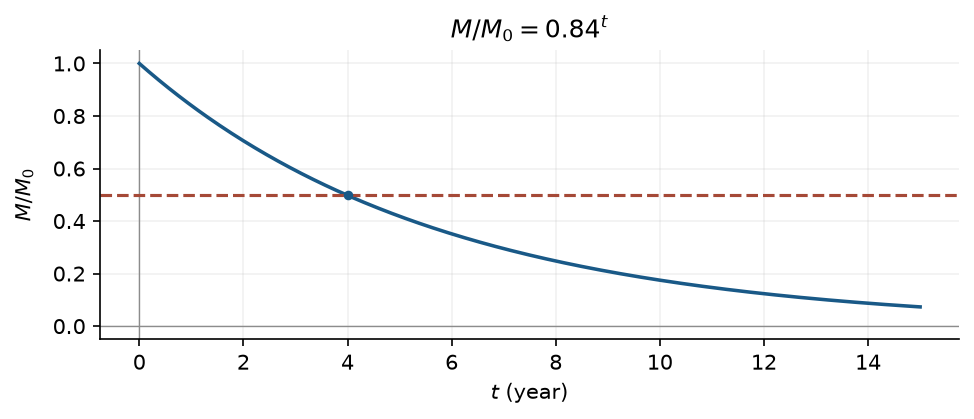
\includegraphics[width=.84\linewidth,height=.38\textheight,keepaspectratio]{figures/C04-EX112-6.png}\end{center}
{\small \field{关联知识}{E03 指数增长、衰减与实际模型（教材帮p.131、132、154 / PDF140、141、163）；F04 函数三种表示法、图象与读数（教材帮p.85、86、93、94 / PDF94、95、102、103）}
\field{方法与易错点}{确认初始量、时间单位、倍率与时刻起点，再代入或逐次比较阈值。 易错：把年折旧10\%写成乘0.1；“超过”用成“达到”；时间起点错一位；把衰减至接近0当实际为0。}
\field{答案依据}{例题原解位置：湘教版教材p.112及题库原图；独立编写可编辑参考解答。答案册此部分主要收练习、习题，不伪造例题答案册位置。}}
